%
% hermite.tex
%
% (c) 2020 Prof Dr Andreas Müller, Hochschule Rapperswil
%
\begin{frame}
\frametitle{Hermite-Polynome}
\vspace{-15pt}
\begin{columns}[t]
\begin{column}{0.3\hsize}
\vspace{-10pt}
\begin{align*}
h_0(x)
&=
(2x+1)(x-1)^2
\\
h_0(0)&=1,\quad h_0(1)=0
%\\
%h_0'(0)&=h_0'(1)=0
\\[5pt]
h_1(x)
&=
x^2(2x-3)
\\
h_1(0)&=0,\quad h_1(1)=1
%\\
%h_1'(0)&=h_1'(1)=0
\\[5pt]
h_i'(0)&=h_i'(1)=0
\\[15pt]
h_0^1(x)
&=
x(x-1)^2
\\
h_0^{1\prime}(0)&=0,\quad h_0^{1\prime}(1)=1
\\[5pt]
h_1^1(x)
&=
x^2(x-1)
\\
h_1^{1\prime}(0)&=1,\quad h_1^{1\prime}(1)=0
\\[5pt]
h_i^1(0)&=h_i^1(1)=0
\end{align*}
\end{column}
\begin{column}{0.66\hsize}
\vspace{-10pt}
\begin{center}
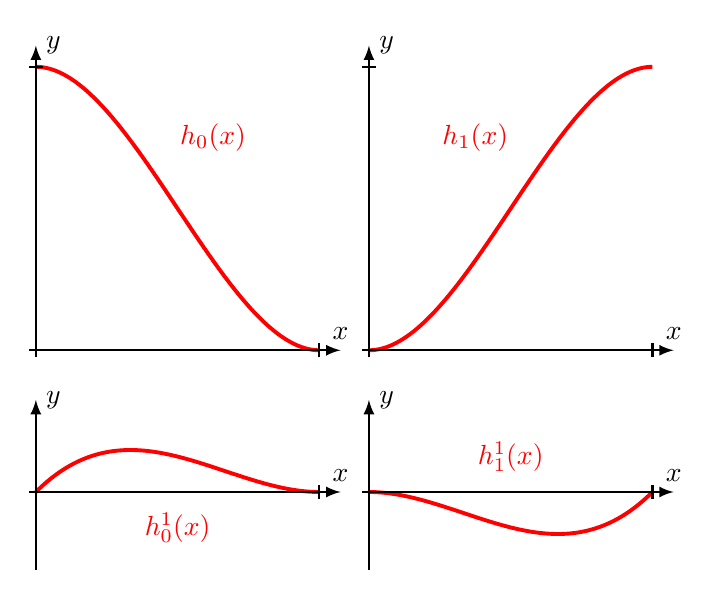
\begin{tikzpicture}[>=latex,thick,scale=0.9]

\begin{scope}
\node[color=red] at (2.5,3) {$h_0(x)$};
\draw[color=red,line width=1.4pt]
	plot[domain=0:1,samples=100]
		({4*\x},{4*(\x-1)*(\x-1)*(2*\x+1)});
\draw[->] (-0.1,0)--(4.3,0) coordinate[label={$x$}];
\draw[->] (0,-0.1)--(0,4.3) coordinate[label={right:$y$}];
\draw (4,-0.1)--(4,0.1);
\draw (-0.1,4)--(0.1,4);
\end{scope}

\begin{scope}[xshift=4.7cm]
\node[color=red] at (1.5,3) {$h_1(x)$};
\draw[color=red,line width=1.4pt]
	plot[domain=0:1,samples=100]
		({4*(1-\x)},{4*(\x-1)*(\x-1)*(2*\x+1)});
\draw[->] (-0.1,0)--(4.3,0) coordinate[label={$x$}];
\draw[->] (0,-0.1)--(0,4.3) coordinate[label={right:$y$}];
\draw (4,-0.1)--(4,0.1);
\draw (-0.1,4)--(0.1,4);
\end{scope}

\begin{scope}[yshift=-2cm]
\node[color=red] at (2,-0.5) {$h_0^1(x)$};
\draw[color=red,line width=1.4pt]
	plot[domain=0:1,samples=100]
		({4*\x},{4*(\x-1)*(\x-1)*\x});
\draw[->] (-0.1,0)--(4.3,0) coordinate[label={$x$}];
\draw[->] (0,-1.1)--(0,1.3) coordinate[label={right:$y$}];
\draw (4,-0.1)--(4,0.1);
\end{scope}

\begin{scope}[xshift=4.7cm,yshift=-2cm]
\node[color=red] at (2,0.5) {$h_1^1(x)$};
\draw[color=red,line width=1.4pt]
	plot[domain=0:1,samples=100]
		({4*\x},{4*\x*\x*(\x-1)});
\draw[->] (-0.1,0)--(4.3,0) coordinate[label={$x$}];
\draw[->] (0,-1.1)--(0,1.3) coordinate[label={right:$y$}];
\draw (4,-0.1)--(4,0.1);
\end{scope}

\end{tikzpicture}
\end{center}
\end{column}
\end{columns}
\end{frame}
